% ------------------------------------------------------------------------------
% TYPO3 CMS 6.2 LTS - What's New - Chapter "Responsive Images" (French Version)
%
% @author	Paul Blondiaux <pblondiaux@sodifrance.fr>
% @author	Philippe Herault <philippe.herault@plan-net.fr>
% @license	Creative Commons BY-NC-SA 3.0
% @link		http://typo3.org/download/release-notes/whats-new/
% @language	French
% ------------------------------------------------------------------------------
% Chapter: Responsive Images
% ------------------------------------------------------------------------------

\section{Responsive Images}
\begin{frame}[fragile]
	\frametitle{Images « Responsive »}

	\begin{center}\huge{Chapitre 2 :}\end{center}
	\begin{center}\huge{\color{typo3darkgrey}\textbf{Images « Responsive »}}\end{center}

\end{frame}

% ------------------------------------------------------------------------------
% Select Screen Size In Page Preview
% ------------------------------------------------------------------------------

\begin{frame}[fragile]
	\frametitle{Images « Responsive »}
	\framesubtitle{Sélectionner une taille d'écran dans la prévisualisation de la page}

	\begin{itemize}
		\item Les contributeurs peuvent sélectionner différentes tailles d'écran dans le module « View » pour tester les sites « Responsive »
	\end{itemize}

	\begin{figure}
		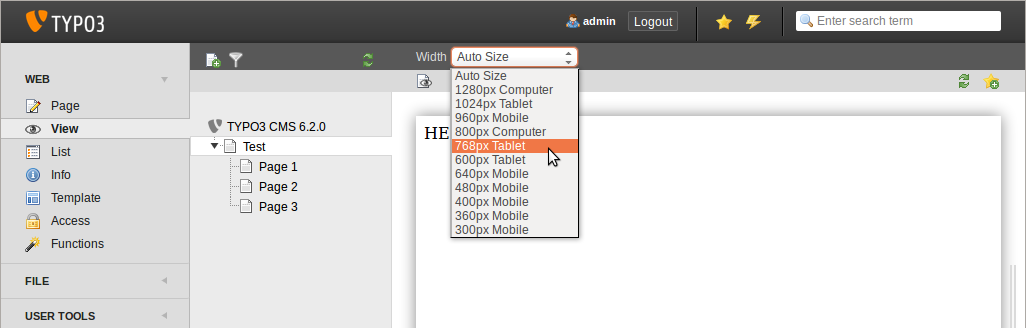
\includegraphics[width=0.95\linewidth]{Images/ResponsiveImages/ScreenSizeInPagePreview.png}
	\end{figure}

\end{frame}

% ------------------------------------------------------------------------------
% Customize Available Screen Sizes
% ------------------------------------------------------------------------------

\begin{frame}[fragile]
	\frametitle{Images « Responsive »}
	\framesubtitle{Personnaliser les tailles d'écran disponibles}

	\begin{itemize}
		\item Les tailles d'écran sont configurables en PageTSconfig :

		\lstset{
			basicstyle=\fontsize{7}{9}\selectfont\ttfamily
		}

		\begin{lstlisting}
			mod.web_view.previewFrameWidths {
			  1780.label = <any LLL or string>
			  1780.height = 145
			}
		\end{lstlisting}

		\item La largeur est définie par une variable (ici : 1780), la hauteur est optionnelle
		\item Des tailles prédéfinies sont disponibles dans :\newline
			\small\texttt{typo3/sysext/core/Configuration/DefaultConfiguration.php}\normalsize
		\item Les libellés peuvent être définis en PageTSconfig :

		\begin{lstlisting}
			mod.web_view.previewFrameWidths {
			  1280.label = LLL:EXT:viewpage/Resources/Private/Language/locallang.xlf:computer
			  1024.label = LLL:EXT:viewpage/Resources/Private/Language/locallang.xlf:tablet
			}
		\end{lstlisting}

	\end{itemize}

\end{frame}

% ------------------------------------------------------------------------------
% Responsive Image Galleries
% ------------------------------------------------------------------------------

\begin{frame}[fragile]
	\frametitle{Images « Responsive »}
	\framesubtitle{Galeries d'images « Responsive »}

	\begin{itemize}
		\item Attributs additionnels pour implémenter des galeries d'images « Responsive »
		\item L'extension « CSS styled content » a été enrichie
		\item Exemple: HTML5 (nécessite \texttt{config.doctype = html5})\newline

			TYPO3 CMS < 6.2:

			\lstset{
				basicstyle=\fontsize{7}{9}\selectfont\ttfamily
			}

			\begin{lstlisting}
				<div class="csc-textpic-imagewrap">...</div>
			\end{lstlisting}

			TYPO3 CMS >= 6.2:

			\begin{lstlisting}
				<div class="csc-textpic-imagewrap"
				  data-csc-images="{register:imageCount}"
				  data-csc-cols="{field:imagecols}">...</div>
			\end{lstlisting}

	\end{itemize}

\end{frame}

% ------------------------------------------------------------------------------
% Responsive Image Rendering
% ------------------------------------------------------------------------------

\begin{frame}[fragile]
	\frametitle{Images « Responsive »}
	\framesubtitle{Rendu des images « Responsive »}

	\begin{itemize}
		\item cObject IMAGE fournit un « sourceCollection » pour supporter diverses résolutions d'écran
		\item Le rendu des images pour les cObjects « texte/image » et « image » nécessite deux paramétrages dans l'éditeur de constantes :

			\texttt{styles.content.imgtext.responsive}\newline
			\texttt{styles.content.imgtext.layoutKey}

		\item Les options « clé en main » sont :

			\begin{itemize}
				\item \texttt{default} :	\tabto{2cm} balise \texttt{<img>} par défaut
				\item \texttt{srcset} :	\tabto{2cm} balise \texttt{<img>} avec les sources alternatives à l'aide de l'attribut \texttt{srcset}
				\item \texttt{picture} :	\tabto{2cm} balise \texttt{<picture>} avec les balises enfant \texttt{source}
				\item \texttt{data} :	\tabto{2cm} balise \texttt{<img>} avec les sources alternatives à l'aide d'attributs \texttt{data}
			\end{itemize}

	\end{itemize}

\end{frame}

% ------------------------------------------------------------------------------
% Property: layoutKey
% ------------------------------------------------------------------------------

\begin{frame}[fragile]
	\frametitle{Images « Responsive »}
	\framesubtitle{Propriété : layoutKey}

	\begin{itemize}
		\item \texttt{layoutKey} définit la disposition\newline
			(il s'agit du code HTML utilisé pour la balise \texttt{<img>})
		\item Chaque option présente un comportement unique pour le rendu HTML
		\item l'option \texttt{default} produit une balise \texttt{<img>} classique\newline
			(à utiliser si le frontend n'est pas « Responsive »)
		\item L'implémentation d'un gabarit « Responsive » nécessite plusieurs tailles d'images pour les différentes résolutions et tailles d'écran
		\item Selon le framework HTML, les capacités du navigateur et les bibliothèques JavaScript (pour une amélioration progressive) :

			\begin{itemize}
				\item utilisez un des gabarits préconfigurés ou
				\item définissez le vôtre
			\end{itemize}

	\end{itemize}

\end{frame}

% ------------------------------------------------------------------------------
% Property: layout
% ------------------------------------------------------------------------------

\begin{frame}[fragile]
	\frametitle{Images « Responsive »}
	\framesubtitle{Propriété : layout}

	\lstset{
		basicstyle=\tiny\ttfamily
	}

	\begin{lstlisting}
		layoutKey = {$styles.content.imgtext.layoutKey}
		layout {
		  default {
		    element = <img src="###SRC###" width="###WIDTH###" height="###HEIGHT###" ###PARAMS###
		      ###ALTPARAMS### ###BORDER######SELFCLOSINGTAGSLASH###>
		  }
		  srcset {
		    element = <img src="###SRC###" srcset="###SOURCECOLLECTION###" ###PARAMS###
		      ###ALTPARAMS### ###SELFCLOSINGTAGSLASH###>
		    source = |*|###SRC### ###SRCSETCANDIDATE###,|*|###SRC### ###SRCSETCANDIDATE###
		  }
		  picture {
		    element = <picture>###SOURCECOLLECTION###<img src="###SRC###" ###PARAMS###
		      ###ALTPARAMS######SELFCLOSINGTAGSLASH###></picture>
		    source = <source src="###SRC###" media="###MEDIAQUERY###"###SELFCLOSINGTAGSLASH###>
		  }
		  data {
		    element = <img src="###SRC###" ###SOURCECOLLECTION### ###PARAMS###
		      ###ALTPARAMS######SELFCLOSINGTAGSLASH###>
		    source = data-###DATAKEY###="###SRC###"
		  }
		}
	\end{lstlisting}

\end{frame}

% ------------------------------------------------------------------------------
% Property: layout.[layoutKey].element
% ------------------------------------------------------------------------------

\begin{frame}[fragile]
	\frametitle{Images « Responsive »}
	\framesubtitle{Propriété : layout.[layoutKey].element}

	\begin{itemize}
		\item \lstinline!###SRC###!\newline
			URL pour l'attribut : \texttt{src}

		\item \lstinline!###WIDTH###!\newline
			Largeur (en pixel) pour l'attribut : \texttt{width}

		\item \lstinline!###HEIGHT###!\newline
			Hauteur (en pixel) pour l'attribut : \texttt{height}

		\item \lstinline!###PARAMS###!\newline
			Paramètres additionnels tels que définis dans le cObject « IMAGE »

		\item \lstinline!###ALTPARAMS###!\newline
			Paramètres additionnels alternatifs tels que définis dans le cObject « IMAGE »
	\end{itemize}

\end{frame}

% ------------------------------------------------------------------------------
% Property: layout.[layoutKey].element
% ------------------------------------------------------------------------------

\begin{frame}[fragile]
	\frametitle{Images « Responsive »}
	\framesubtitle{Propriété : layout.[layoutKey].element}

	\begin{itemize}
		\item \lstinline!###BORDER###!\newline
			Bordure (en pixel) pour l'attribut : \texttt{border}

		\item \lstinline!###SELFCLOSINGTAGSLASH###!\newline
			Balise fermante, par exemple : \texttt{<img ... />} vs. \texttt{<img ... >}\newline
			(dépend de \texttt{config.xhtmlDoctype} ou de \texttt{config.doctype})

		\item \lstinline!###SOURCECOLLECTION###!\newline
			Images sources additionnelles, dépend du design web « Responsive » utilisé.
			Les valeurs exactes sont définies dans : \texttt{layout.[layoutKey].source}
	\end{itemize}

\end{frame}

% ------------------------------------------------------------------------------
% Property: sourceCollection.[dataKey]
% ------------------------------------------------------------------------------

\begin{frame}[fragile]
	\frametitle{Images « Responsive »}
	\framesubtitle{Propriété : sourceCollection.[dataKey]}

	\begin{itemize}
		\item « sourceCollection » par défaut de EXT:css\_styled\_content
		\item Créer votre propre « sourceCollection » est vivement recommandé

			\lstset{
				basicstyle=\tiny\ttfamily
			}

			\begin{lstlisting}
				sourceCollection {
				  small {
				    width = 200
				    srcsetCandidate = 600w
				    mediaQuery = (max-device-width: 600px)
				    dataKey = small
				  }
				  smallRetina {
				    if.directReturn = 1
				    width = 200
				    pixelDensity = 2
				    srcsetCandidate = 600w 2x
				    mediaQuery = (max-device-width: 600px) AND (min-resolution: 192dpi)
				    dataKey = smallRetina
				  }
				}
			\end{lstlisting}
	\end{itemize}

\end{frame}

% ------------------------------------------------------------------------------
% Further Resources (External Links)
% ------------------------------------------------------------------------------

\begin{frame}[fragile]
	\frametitle{Images « Responsive »}
	\framesubtitle{Aller plus loin}

	\begin{itemize}
		\item Exemple de code fonctionnel :\newline
			\small\url{http://wiki.typo3.org/Responsive_Image_Rendering}\normalsize

		\item Article de Sven Wolfermann sur typo3.org :\newline
			\small\url{http://typo3.org/news/article/responsive-image-rendering-in-typo3-cms-62/}\normalsize

		\item Spécifications du W3C :\newline
			\small\url{http://www.w3.org/html/wg/drafts/srcset/w3c-srcset/}\newline
			\small\url{http://www.w3.org/TR/html-picture-element/}\normalsize

		\item Brouillon fonctionnel du « Responsive Image Community Group » :\newline
			\small\url{http://responsiveimages.org}\normalsize

	\end{itemize}

\end{frame}

% ------------------------------------------------------------------------------

